\documentclass[11pt,a4paper]{article}
\usepackage[utf8]{inputenc}
\usepackage[T1]{fontenc}
\usepackage[english]{babel}
\usepackage{lmodern,microtype}
\usepackage[a4paper,margin=1.8cm,top=1.6cm,bottom=1.7cm]{geometry}
\usepackage{booktabs,tabularx,longtable,array,xcolor,amsmath,graphicx}
\usepackage[hidelinks]{hyperref}
\usepackage{titlesec,fancyhdr}
\definecolor{azul}{HTML}{173B56}
\titleformat{\section}{\large\bfseries\color{azul}}{\thesection.}{0.5em}{}
\titlespacing*{\section}{0pt}{10pt}{7pt}
\setlength{\parindent}{0pt}
\setlength{\parskip}{7pt}
\setlength{\emergencystretch}{2em}
\pagestyle{fancy}\fancyhf{}\fancyfoot[R]{\small\thepage}
\renewcommand{\headrulewidth}{0pt}
\newcolumntype{Y}{>{\raggedright\arraybackslash}X}

\begin{document}
{\LARGE\bfseries\color{azul} Executive report}\par
{\small Unsupervised learning for DataCo commercial and operational data}

\section{Problem, dataset, and preprocessing decisions}
Commercial data combine customers, products, sales, discounts, profitability, and shipping. Their volume and interrelated features make transaction profiles, latent factors, and atypical observations difficult to characterize through descriptive statistics alone. Transactions with similar sales can have different margins, while unusual behavior can reflect either favorable or adverse business outcomes. This study therefore addresses the following question:

\begingroup\leftskip=10pt\rightskip=10pt
\textbf{What structures, relationships, and latent patterns can unsupervised learning identify in commercial and operational order data, and to what extent can these methods characterize commercial profiles, explore customer--product affinities, and identify atypical behavior?}\par
\endgroup

The \textbf{DataCo} supply-chain dataset originally contained \textbf{180,519 records and 53 features}. Each record represents an order item, so multiple records may belong to one order. Attributes cover products, customers, geography, sales, discounts, profits, and shipping times.

Preprocessing removed insufficient-information fields, including the entirely empty \textit{Product Description} and \textit{Order Zipcode}, with approximately 86.24\% missing values. Constant columns, redundant attributes, order/item identifiers, and unnecessary personal information were also removed. Customer and product identifiers were retained for interaction analysis; \textit{Order Month} was extracted from the order date. Negative profitability was retained as commercially plausible loss. No duplicate rows were found and no observations were removed.

The processed dataset contained \textbf{180,519 records and 33 features}. Most numerical models used ten features describing actual/scheduled shipping duration, profit, sales, discounts, profit ratio, quantity, and price. GMM used a four-feature subset for interpretable profiles; recommendation used customer--product interactions.

\section{Methods, hyperparameters, and validation criteria}
Methods addressed complementary objectives: probabilistic profiles, latent representations, nonlinear relationships, recommendation, and atypical observations. Task-specific evaluation combined quantitative performance, stability, and business interpretation. Selection balanced representation quality and complexity rather than assuming one technique was best for every objective.

\begingroup
\fontsize{9}{10.8}\selectfont
\setlength{\tabcolsep}{5pt}\renewcommand{\arraystretch}{1.12}
\setlength{\LTpre}{0pt}\setlength{\LTpost}{5pt}
\begin{longtable}{@{}>{\raggedright\arraybackslash}p{2.55cm}*{2}{>{\raggedright\arraybackslash}p{\dimexpr(\textwidth-2.55cm-4\tabcolsep)/2\relax}}@{}}
\toprule
\textbf{Objective and models} & \textbf{Selected configuration} & \textbf{Selection and validation}\\
\midrule\endfirsthead
\toprule
\textbf{Objective and models} & \textbf{Selected configuration} & \textbf{Selection and validation}\\
\midrule\endhead
\midrule\endfoot\bottomrule\endlastfoot
Profiles: GMM & Four components, diagonal covariance, ten initializations. Sales, discount rate, profit ratio, and quantity. & 32 configurations; AIC, BIC, log-likelihood, silhouette, Davies--Bouldin, Calinski--Harabasz, interpretation, and ARI across ten seeds.\\[4pt]
Reduction: SVD, PCA, PPCA & Five components per method, exploring one to nine. & MSE, relative Frobenius error, retained energy/variance, subspace stability with ten bootstrap samples, interpretation; PPCA log-likelihood.\\[4pt]
Factors: FA, ICA & FA: five factors and varimax rotation. ICA: five components, unit-variance whitening. & Reconstruction, recovered energy, bootstrap stability, coefficient concentration, convergence, and interpretation.\\[4pt]
Recommendation: SVD & Two latent factors, Top-10 lists; comparison with a popularity baseline. & HitRate@10 and NDCG@10 on held-out validation and test interactions.\\[4pt]
Visualization: t-SNE, UMAP & Two dimensions. t-SNE: perplexity=30. UMAP: n\_neighbors=30, min\_dist=0.1. & Trustworthiness and overlap at $k=2,5,10,30,50$; global distance Spearman; neighbor stability across ten seeds.\\[4pt]
Anomalies: PCA, ICA, Mahalanobis & PCA/ICA: five components. ICA: Gaussian KDE, bandwidth=0.3, 5,000 observations. Mahalanobis: Ledoit--Wolf covariance. & $T^2$, SPE, NLL, and squared-distance scores; training-derived thresholds and descriptive flagged/non-flagged comparisons.\\[4pt]
Anomalies: LOF, IF & LOF: twenty neighbors. Final IF: 400 trees, 1,024 observations per tree. & Hyperparameter sensitivity, score Spearman, Jaccard of the most extreme 1\%. LOF: resampling; IF: seeds.\\[4pt]
Networks: AE, VAE & AE: five dimensions, hidden width 64, learning rate=0.001, batch size 128. VAE: five dimensions, hidden width 64, $\beta=0.001$, learning rate=0.001, batch size 256. & AE: validation MSE, latent CKA, reconstruction RMSE. VAE: MSE+$\beta\cdot$KL. Adam, early stopping, and stability across ten seeds.\\[4pt]
Associations: Apriori & Minimum support 0.05, confidence 0.50; lift greater than 1. Binary customer--product matrix. & Support, confidence, lift across purchase histories; no temporal sequence or causal effect is established.\\
\end{longtable}
\endgroup

\begingroup\fontsize{10}{12}\selectfont
GMM used \textbf{80\%/20\%} training/validation partitions. Reduction and factor methods used \textbf{70\%/15\%/15\%}; anomaly models and networks used \textbf{60\%/20\%/20\%} training/validation/test partitions. Recommendation held out interactions; embedding hyperparameters were evaluated on \textbf{30,000 observations}. Scaling was fitted on training data where applicable: SVD without centering, other numerical models with centered standardization. Exploratory t-SNE/UMAP fitted scaling on the full data.

Anomalies were flagged above the \textbf{95th and 99th percentiles of training scores} ($\alpha=0.05$ and $\alpha=0.01$). These criteria vary selection breadth without confirming errors or threats. Without verified labels, evaluation focused on stability, sensitivity, and descriptive interpretation rather than accuracy or false-positive/false-negative rates.\par
\endgroup

\section{Comparative results and interpretation}
\textbf{Commercial profiles and latent representations.} GMM identified mostly profitable single-item purchases (53\%), small two-item purchases (10\%), loss-making transactions (5.8\%), and mostly profitable multi-item purchases (30\%). SVD, PCA, and PPCA recovered similar themes of transaction value, profitability, discounts, shipping, and quantity--price. PCA and PPCA were particularly similar; uncentered SVD mixed some contributions more strongly. FA and ICA recovered related themes with axes and weights partly different from PCA. All supported descriptive business interpretations without demonstrating causality.

\begingroup\fontsize{8.3}{10}\selectfont
\setlength{\tabcolsep}{3pt}\renewcommand{\arraystretch}{1.18}
\setlength{\LTpre}{3pt}\setlength{\LTpost}{4pt}
\begin{longtable}{@{}>{\raggedright\arraybackslash}p{1.1cm}*{5}{>{\raggedright\arraybackslash}p{\dimexpr(\textwidth-1.1cm-10\tabcolsep)/5\relax}}@{}}
\toprule
\textbf{Model} & \textbf{Dimension 1} & \textbf{Dimension 2} & \textbf{Dimension 3} & \textbf{Dimension 4} & \textbf{Dimension 5}\\
\midrule\endfirsthead
\toprule
\textbf{Model} & \textbf{Dimension 1} & \textbf{Dimension 2} & \textbf{Dimension 3} & \textbf{Dimension 4} & \textbf{Dimension 5}\\
\midrule\endhead
\midrule\endfoot\bottomrule\endlastfoot
SVD & Longer shipping and greater transaction activity. & Higher value/price, shorter shipping, lower quantity. & Higher profit and profit ratio. & Greater discounts, shorter shipping. & More units of inexpensive products.\\[3pt]
PCA & Higher sales/prices and absolute discounts. & Higher profit and profit ratio. & Longer actual and scheduled shipping. & Greater discounts, relatively low sales/prices. & More units, lower price and discount rate.\\[3pt]
PPCA & Higher sales and prices. & Higher profit and profit ratio. & Longer actual and scheduled shipping. & Greater discounts, lower price and sales per customer. & More units, lower price and discount rate.\\[3pt]
FA & Higher transaction value and price. & Greater discount intensity. & Higher price and lower quantity. & Lower profit and profit ratio. & Shorter actual and scheduled shipping.\\[3pt]
ICA & Greater discount intensity. & Lower profit and profit ratio. & Higher price and lower quantity. & Longer actual and scheduled shipping. & Higher value, price, and absolute discounts.\\[3pt]
AE & Greater discounts, longer shipping, higher price. & More units, lower price, longer shipping. & More units, lower price, shorter shipping. & Lower quantity and sales. & Higher profitability and shorter shipping.\\
\end{longtable}\par
\textit{Reading:} cells describe patterns associated with high scores in the selected model. Axis order/sign can change; dimensions are not order categories. AE interpretation examines features that increase/decrease with each dimension, rather than causal effects or exact network contributions.
\endgroup

\begin{center}\begin{minipage}{\linewidth}\centering
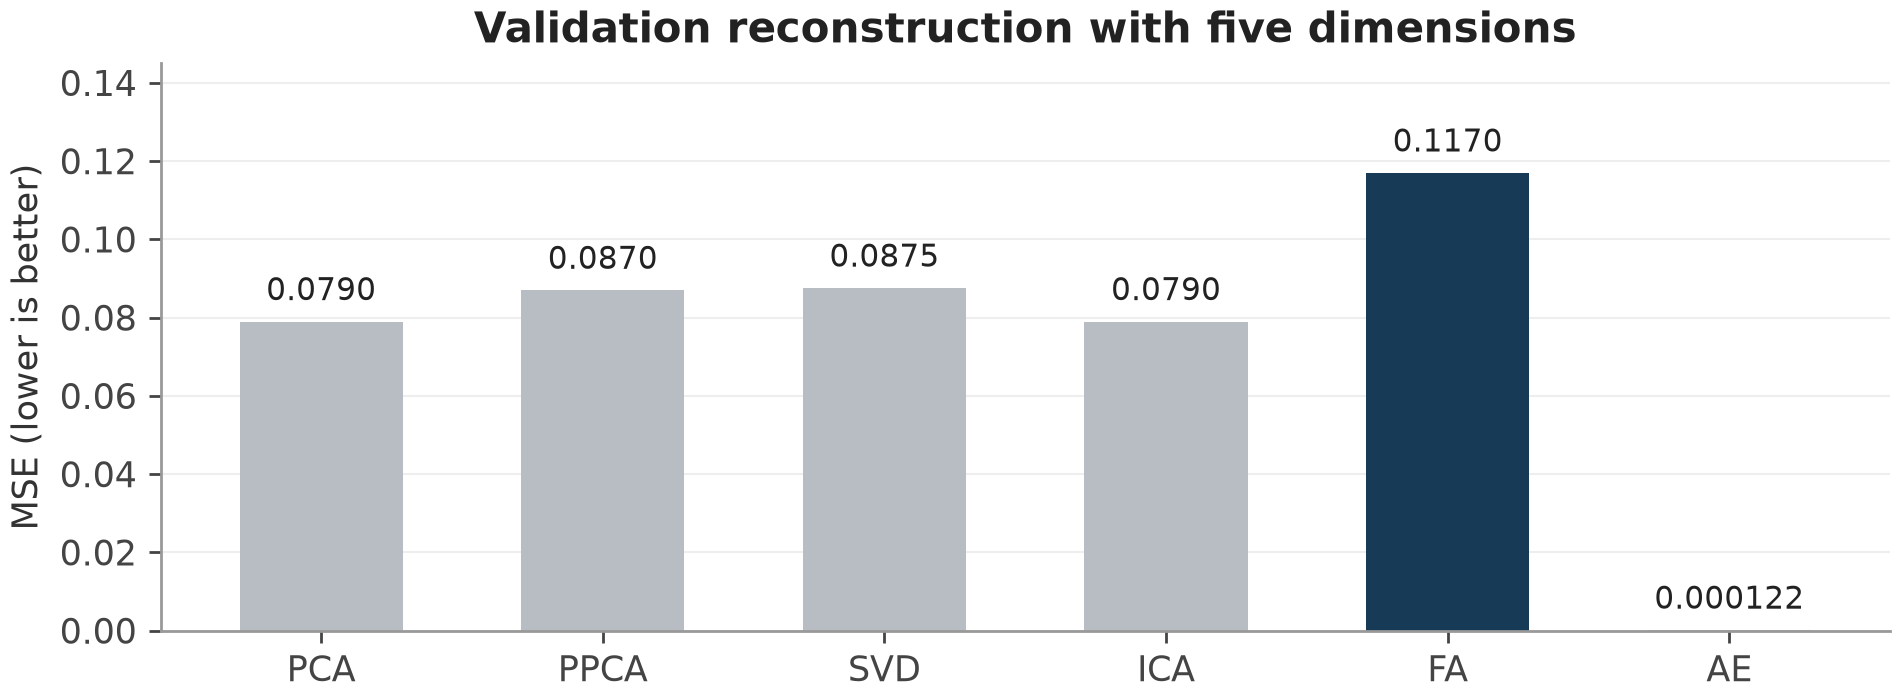
\includegraphics[width=0.94\linewidth]{figuras/en/05_reconstruccion_todos_modelos.png}\par
{\footnotesize\textbf{Figure 1.} FA is highlighted for the highest MSE, not the best performance. All use five dimensions; SVD is uncentered and AE uses a different split (60/20/20 versus 70/15/15). This is descriptive, not a controlled ranking of superiority.}
\end{minipage}\end{center}

AE shared themes with linear methods but combined them differently: AE1 linked discounts and long shipping; AE2--AE3, quantity and lower price; AE4, lower quantity and sales; AE5, profitability and short shipping. Interpretation refers to the selected model and was seed-sensitive.

\textbf{Recommendation, visualization, and associations.} Popularity outperformed two-factor SVD in test HitRate@10 (0.8507 versus 0.8298) and NDCG@10 (0.6572 versus 0.5810). Twenty products accounted for about 82\% of interactions. t-SNE better preserved close neighbors (overlap@10 around 0.74), whereas UMAP better preserved global distance ordering than the selected t-SNE (Spearman 0.315 versus 0.13), although both correlations were limited. Shipping Mode showed the clearest segmentation; products/categories had localized concentrations. Apriori produced 511 frequent itemsets and 9,206 rules; the top ten partitioned the same nine products, with 6.18\% support, 50--58\% confidence, and 2.55--2.60 lift. Associations can inform campaigns without proving incremental sales.

\textbf{Documented example: rule 9205.} $A\Rightarrow B$, using abbreviated names: $A$ contains Nike Free, Under Armour toddler shoes, Diamondback Serene bike, and Pelican Sunstream kayak; $B$ contains Perfect Fitness Rip Deck, Nike CJ Elite cleats, Nike Dri-FIT polo, Field \& Stream safe, and O'Brien vest. \textbf{Support 6.18\%}: this proportion of customers purchased all nine products. \textbf{Confidence 54.44\%}: among customers purchasing every item in $A$, this proportion also purchased every item in $B$. \textbf{Lift 2.60}: purchasing the complete $B$ set was 2.60 times as prevalent among $A$ purchasers as among all customers. This establishes neither temporal order nor causality.

\begin{center}\begin{minipage}{\linewidth}\centering
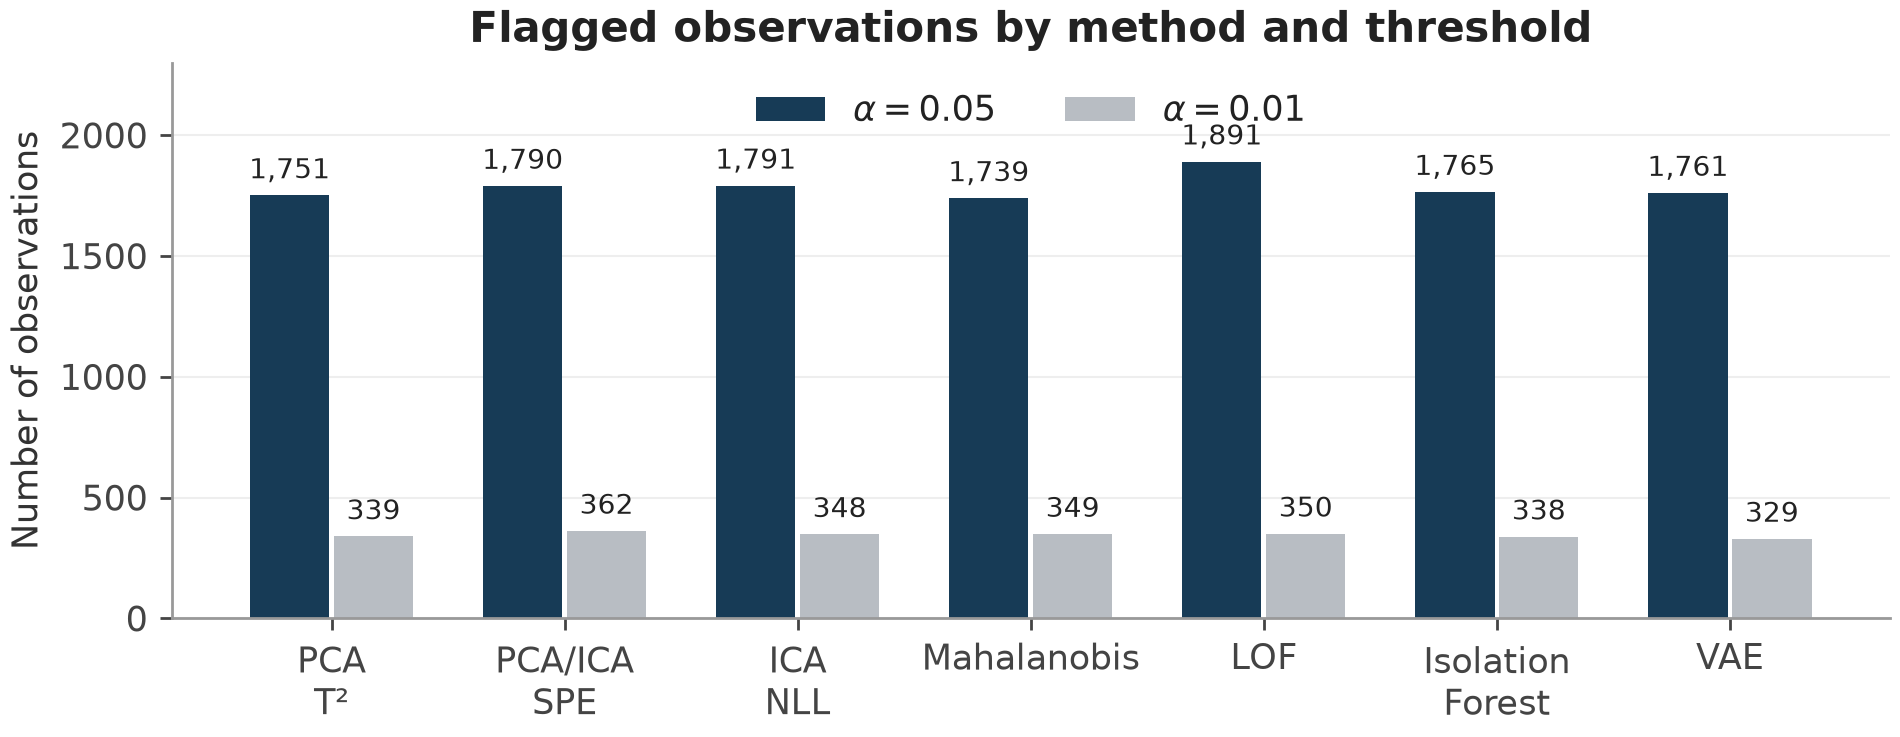
\includegraphics[width=0.94\linewidth]{figuras/en/06_conteo_anomalias_metodos.png}\par
{\footnotesize\textbf{Figure 2.} Validation: 36,104 records; training-derived thresholds. PCA and ICA--SPE are grouped because results coincide. Counts overlap and should not be added together.}
\end{minipage}\end{center}

\textbf{Atypicality and threshold selection.} Within each threshold, counts were similar: 1,739--1,891 at 5\% and 329--362 at 1\%, including VAE. This implies neither identical detections nor equal accuracy. Flagged observations included losses, high profits, and unusual combinations of sales, discounts, quantity, and shipping. Atypicality does not imply business harm, and high profit does not rule out operational problems.

No verified anomaly labels are available. Raising the threshold reduces detections and can increase false negatives; lowering it broadens detections and can increase false positives. These rates were not measured and are not represented by $\alpha$. We recommend $\alpha=0.05$ for \emph{exploration}: it permits reviewing a potentially broader variety of cases, including less extreme observations than $\alpha=0.01$, without establishing greater accuracy.

\section{Conclusions, limitations, biases, and future work}
\textbf{Conclusions.} Methods were complementary: GMM characterized probabilistic profiles, latent representations summarized interpretable commercial dimensions, and t-SNE/UMAP supported similarity exploration. Reconstruction, stability, and interpretability require separate assessment. Popularity outperformed the implemented SVD recommender; rules provided exploratory cross-selling associations. Anomalies represent statistical atypicality rather than confirmed harm and should be prioritized against business objectives.

\textbf{Limitations and biases.} Unavailable labels prevented measurement of detection accuracy and errors. Results depend on features, scaling, parameters, seeds, and thresholds. Changing t-SNE/UMAP inputs can alter neighbors/groupings; color overlays only contextualize the map. Related monetary features can reinforce patterns. Popularity, customer activity, and uneven dataset coverage influence recommendations and rules; histories establish neither sequence nor causality. Latent factors are descriptive interpretations, and AE dimensions were sensitive across runs.

\textbf{Future work.} Explain individual anomaly contributions, distinguish beneficial/adverse outcomes, and contextualize them by region, customer, and product. Validate temporal stability, evaluate recommendation diversity/coverage, reduce rule redundancy, complement association analysis with FP-Growth, and test promotions through experiments measuring incremental sales and profitability.
\end{document}
